% This file was created by tikzplotlib v0.9.1.
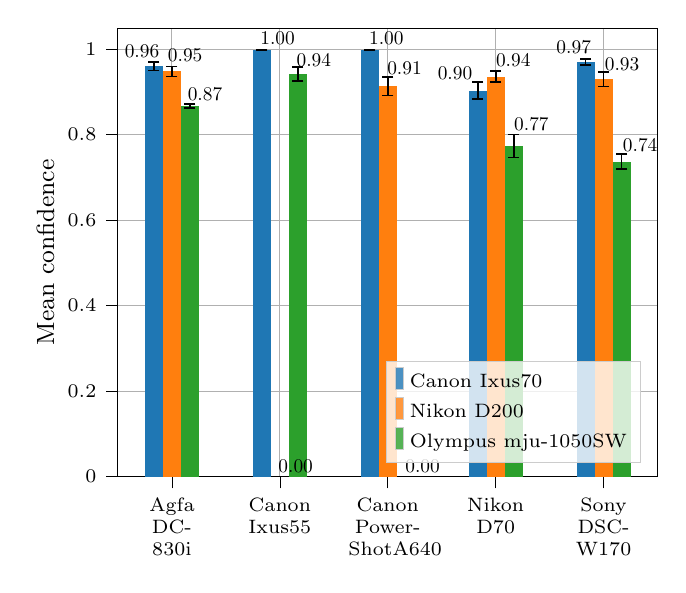
\begin{tikzpicture}

\definecolor{color0}{rgb}{0.12156862745098,0.466666666666667,0.705882352941177}
\definecolor{color1}{rgb}{1,0.498039215686275,0.0549019607843137}
\definecolor{color2}{rgb}{0.172549019607843,0.627450980392157,0.172549019607843}

\pgfplotsset{compat=1.11,
	/pgfplots/ybar legend/.style={
		/pgfplots/legend image code/.code={%
			\draw[##1,/tikz/.cd,yshift=-0.25em]
			(0cm,0cm) rectangle (3pt,0.8em);},
	}, every tick label/.append style={font=\scriptsize}
}

\begin{axis}[
legend cell align={left},
legend style={fill opacity=0.8, draw opacity=1, text opacity=1, at={(0.97,0.03)}, anchor=south east, draw=white!80!black},
tick align=outside,
tick pos=left,
grid=major,
x grid style={white!69.0196078431373!black},
xmin=-0.5, xmax=4.5,
xtick style={color=black},
xtick={0,1,2,3,4},
xticklabel style={text width=1cm, align=center},
xticklabels={Agfa DC-830i,Canon Ixus55,Canon PowerShotA640,Nikon D70,Sony DSC-W170},
y grid style={white!69.0196078431373!black},
ymin=0, ymax=1.04887666648719,
ytick style={color=black},
y label style={at={(axis description cs:-0.1,.5)},anchor=south},
ylabel={\small Mean confidence}
]
\draw[draw=none,fill=color0] (axis cs:-0.25,0) rectangle (axis cs:-0.0833333333333333,0.960057199001312);
\addlegendimage{ybar,ybar legend,draw=none,fill=color0};
\addlegendentry{\scriptsize Canon Ixus70}

\draw[draw=none,fill=color0] (axis cs:0.75,0) rectangle (axis cs:0.916666666666667,0.998571991920471);
\draw[draw=none,fill=color0] (axis cs:1.75,0) rectangle (axis cs:1.91666666666667,0.998243570327759);
\draw[draw=none,fill=color0] (axis cs:2.75,0) rectangle (axis cs:2.91666666666667,0.902838289737701);
\draw[draw=none,fill=color0] (axis cs:3.75,0) rectangle (axis cs:3.91666666666667,0.969556868076324);
\draw[draw=none,fill=color1] (axis cs:-0.0833333333333333,0) rectangle (axis cs:0.0833333333333333,0.947647273540497);
\addlegendimage{ybar,ybar legend,draw=none,fill=color1};
\addlegendentry{\scriptsize Nikon D200}

\draw[draw=none,fill=color1] (axis cs:0.916666666666667,0) rectangle (axis cs:1.08333333333333,0);
\draw[draw=none,fill=color1] (axis cs:1.91666666666667,0) rectangle (axis cs:2.08333333333333,0.912966668605804);
\draw[draw=none,fill=color1] (axis cs:2.91666666666667,0) rectangle (axis cs:3.08333333333333,0.935871481895447);
\draw[draw=none,fill=color1] (axis cs:3.91666666666667,0) rectangle (axis cs:4.08333333333333,0.928948819637299);
\draw[draw=none,fill=color2] (axis cs:0.0833333333333333,0) rectangle (axis cs:0.25,0.867151260375977);
\addlegendimage{ybar,ybar legend,draw=none,fill=color2};
\addlegendentry{\scriptsize Olympus mju-1050SW}

\draw[draw=none,fill=color2] (axis cs:1.08333333333333,0) rectangle (axis cs:1.25,0.941826820373535);
\draw[draw=none,fill=color2] (axis cs:2.08333333333333,0) rectangle (axis cs:2.25,0);
\draw[draw=none,fill=color2] (axis cs:3.08333333333333,0) rectangle (axis cs:3.25,0.773304998874664);
\draw[draw=none,fill=color2] (axis cs:4.08333333333333,0) rectangle (axis cs:4.25,0.736984550952911);
\path [draw=black, semithick]
(axis cs:-0.166666666666667,0.949836290441453)
--(axis cs:-0.166666666666667,0.970278107561171);

\path [draw=black, semithick]
(axis cs:0.833333333333333,0.998213825281709)
--(axis cs:0.833333333333333,0.998930158559233);

\path [draw=black, semithick]
(axis cs:1.83333333333333,0.997746782202739)
--(axis cs:1.83333333333333,0.998740358452778);

\path [draw=black, semithick]
(axis cs:2.83333333333333,0.883183458819985)
--(axis cs:2.83333333333333,0.922493120655417);

\path [draw=black, semithick]
(axis cs:3.83333333333333,0.962237296625972)
--(axis cs:3.83333333333333,0.976876439526677);

\path [draw=black, semithick]
(axis cs:0,0.935686012730002)
--(axis cs:0,0.959608534350991);

\path [draw=black, semithick]
(axis cs:1,0)
--(axis cs:1,0);

\path [draw=black, semithick]
(axis cs:2,0.891556613147259)
--(axis cs:2,0.93437672406435);

\path [draw=black, semithick]
(axis cs:3,0.92278899345547)
--(axis cs:3,0.948953970335424);

\path [draw=black, semithick]
(axis cs:4,0.912190033122897)
--(axis cs:4,0.9457076061517);

\path [draw=black, semithick]
(axis cs:0.166666666666667,0.862032268662006)
--(axis cs:0.166666666666667,0.872270252089947);

\path [draw=black, semithick]
(axis cs:1.16666666666667,0.925926184281707)
--(axis cs:1.16666666666667,0.957727456465364);

\path [draw=black, semithick]
(axis cs:2.16666666666667,0)
--(axis cs:2.16666666666667,0);

\path [draw=black, semithick]
(axis cs:3.16666666666667,0.746303979307413)
--(axis cs:3.16666666666667,0.800306018441916);

\path [draw=black, semithick]
(axis cs:4.16666666666667,0.71960430033505)
--(axis cs:4.16666666666667,0.754364801570773);

\addplot [semithick, black, mark=-, mark size=2, mark options={solid}, only marks]
table {%
-0.166666666666667 0.949836290441453
0.833333333333333 0.998213825281709
1.83333333333333 0.997746782202739
2.83333333333333 0.883183458819985
3.83333333333333 0.962237296625972
};

\addplot [semithick, black, mark=-, mark size=2, mark options={solid}, only marks]
table {%
-0.166666666666667 0.970278107561171
0.833333333333333 0.998930158559233
1.83333333333333 0.998740358452778
2.83333333333333 0.922493120655417
3.83333333333333 0.976876439526677
};

\addplot [semithick, black, mark=-, mark size=2, mark options={solid}, only marks]
table {%
0 0.935686012730002
1 0
2 0.891556613147259
3 0.92278899345547
4 0.912190033122897
};

\addplot [semithick, black, mark=-, mark size=2, mark options={solid}, only marks]
table {%
0 0.959608534350991
1 0
2 0.93437672406435
3 0.948953970335424
4 0.9457076061517
};

\addplot [semithick, black, mark=-, mark size=2, mark options={solid}, only marks]
table {%
0.166666666666667 0.862032268662006
1.16666666666667 0.925926184281707
2.16666666666667 0
3.16666666666667 0.746303979307413
4.16666666666667 0.71960430033505
};

\addplot [semithick, black, mark=-, mark size=2, mark options={solid}, only marks]
table {%
0.166666666666667 0.872270252089947
1.16666666666667 0.957727456465364
2.16666666666667 0
3.16666666666667 0.800306018441916
4.16666666666667 0.754364801570773
};

\draw (axis cs:-0.5,0.98) node[
  scale=0.7,
  anchor=base west,
  text=black,
  rotate=0.0
]{0.96};
\draw (axis cs:0.756,1.01) node[
  scale=0.7,
  anchor=base west,
  text=black,
  rotate=0.0
]{1.00};
\draw (axis cs:1.764,1.01) node[
  scale=0.7,
  anchor=base west,
  text=black,
  rotate=0.0
]{1.00};
\draw (axis cs:2.4,0.93) node[
  scale=0.7,
  anchor=base west,
  text=black,
  rotate=0.0
]{0.90};
\draw (axis cs:3.5,0.99) node[
  scale=0.7,
  anchor=base west,
  text=black,
  rotate=0.0
]{0.97};
\draw (axis cs:-0.1,0.97) node[
  scale=0.7,
  anchor=base west,
  text=black,
  rotate=0.0
]{0.95};
\draw (axis cs:0.924,0.01) node[
  scale=0.7,
  anchor=base west,
  text=black,
  rotate=0.0
]{0.00};
\draw (axis cs:1.932,0.94) node[
  scale=0.7,
  anchor=base west,
  text=black,
  rotate=0.0
]{0.91};
\draw (axis cs:2.94,0.96) node[
  scale=0.7,
  anchor=base west,
  text=black,
  rotate=0.0
]{0.94};
\draw (axis cs:3.948,0.95) node[
  scale=0.7,
  anchor=base west,
  text=black,
  rotate=0.0
]{0.93};
\draw (axis cs:0.084,0.88) node[
  scale=0.7,
  anchor=base west,
  text=black,
  rotate=0.0
]{0.87};
\draw (axis cs:1.092,0.96) node[
  scale=0.7,
  anchor=base west,
  text=black,
  rotate=0.0
]{0.94};
\draw (axis cs:2.1,0.01) node[
  scale=0.7,
  anchor=base west,
  text=black,
  rotate=0.0
]{0.00};
\draw (axis cs:3.108,0.81) node[
  scale=0.7,
  anchor=base west,
  text=black,
  rotate=0.0
]{0.77};
\draw (axis cs:4.116,0.76) node[
  scale=0.7,
  anchor=base west,
  text=black,
  rotate=0.0
]{0.74};
\end{axis}

\end{tikzpicture}
